\chapter{Il Livello Applicazione}
\thispagestyle{chapterInit}
\section{principi delle applicazioni di rete}
    \subsection{Architetture di rete}
        Esistono varie architetture per le applicazioni di rete, tra le quali:
        \begin{itemize}
            \item Client-Server
            \item Peer-to-Peer
            \item Architetture ibride
            \item Cloud Computing 
        \end{itemize}
        \subsubsection{Client - Server}
        \label{subsubsec:clientServer}
            In questa architettura esistono due ruoli principali:
            \paragraph{Server} Il server è un host \textbf{sempre attivo} con un \textbf{indirizzo permanente} e molto spesso difficile da scalare
            \paragraph{Client} Il client \textbf{comunica col server}, inoltre a differenza del server può \textbf{disconnettersi temporaneamente} e inoltre può avere un \textbf{indirizzo IP dinamico}. Generalmente i client \textbf{non comunicano tra di loro}.
        \subsubsection[Architettura P2P pura]{Architettura \Acrshort*{P2P} pura}
            In questa architettura \textbf{non c'è} sempre un server attivo, vengono eseguire \textbf{coppie arbitrarie} di host che comunicano tra di loro. Infine i \textbf{peer} non devono necessariamente essere sempre attivi e possono avere un \textbf{indirizzo IP dinamico}.

        \subsubsection{Architetture ibride}
            In queste architetture si ha una combinazione tra client-server e \Acrshort*{P2P}, ad esempio un server con peer che comunicano tra di loro. Un esempio di architettura ibrida è Skype, oppure un applicativo di messaggistica istantanea dove le chat sono \Acrshort*{P2P} ma l'individuazione degli utenti è fatta tramite un server centrale.
        \subsubsection{Cloud Computing}
            In questa architettura si ha un insieme di tecnologie che permettono \textbf{di memorizzare archiviare e/o elaborare dati} tramite l'utilizzo di risorse distribuite. La creazione di copie di sicurezza dette \textbf{backup} è automatica e l'operabilità si trasferisce online. I dati sono memorizzati in \textbf{server farm} generalmente localizzate nei paesi di origine del service provider.
    \subsection{Struttura delle applicazioni di rete}
        \subsubsection{Processi del sistema operativo}
            \paragraph{Processo} Programma in esecuzione su un host.
            
            All'interno di uno stesso host due processi comunicano utilizzando \textbf{schemi interprocesso} (definiti dal \Acrshort*{SO}).

            Processi su host diversi comunicano tramite \textbf{messaggi} scambiati tramite la rete.
            \paragraph{Processo client} processo che inizia la comunicazione
            \paragraph{Processo server} processo che attende di essere contattato
        \subsubsection{Socket}
            \paragraph{Socket} Astrazione software che permette ad un processo di inviare e ricevere messaggi da un altro processo attraverso la rete.\newline
            Una \textit{socket} è analoga ad una porta (il processo fà uscire il messaggio dalla sua porta e il messaggio entra dalla porta del processo destinatario).

    \subsection{Indirizzamento}
        \paragraph{\Acrshort*{IP}} Per identificare un host in modo univoco si usa un \textbf{indirizzo \Acrshort*{IP}} che è formato da 32 bit. 

        \paragraph{Numeri di porta} L'indirizzo \Acrshort*{IP} però non è sufficiente ad identificare un processo all'interno dell'\textit{host} per questo definiamo dei \textbf{numeri di porta}.

    \subsection{Protocolli a livello applicazione}
        \subsubsection{Definizioni}
            I protocolli a livello applicazione definiscono:
                \begin{itemize}
                    \item Tipi di messaggi scambiati
                    \item Sintassi dei messaggi
                    \item Semantica dei campi dei messaggi
                    \item Regole per determinare quando e come i processi inviano e ricevono messaggi
                \end{itemize}
            \paragraph{Protocolli dominio pubblico}Alcuni protocolli sono di pubblico dominio definiti nelle \acrfull*{RFC} della \acrfull*{IETF}. Questi consentono interoperabilità tra diversi host, esempi di protocolli a pubblico dominio sono: \Acrshort*{HTTP}, \Acrshort*{SMTP}\dots
            \paragraph{Protocolli proprietari} Altri protocolli sono proprietari, ad esempio Skype.
    \subsection{Servizi di trasporto}
        \subsubsection{Come segliere il protocollo di trasporto}
            \begin{description}
                \item[Perdita di dati] Applicazioni che richiedono trasmissione affidabile dei dati (es. \textit{file transfer}) richiedono un protocollo di trasporto affidabile
                \item[Temporizzazione] Applicazioni che richiedono bassa latenza (es. \Acrshort*{VoIP}) richiedono un protocollo di trasporto con bassa temporizzazione
                \item[Throughput] Applicazioni che richiedono alto throughput richiedono un protocollo di trasporto con alto throughput
                \item[Sicurezza] Applicazioni che richiedono sicurezza (es. trasferimento di file) richiedono un protocollo di trasporto sicuro
            \end{description}
            \begin{table}[H]
                \centering
                \begin{adjustbox}{max width=\textwidth}
                    \begin{tabular}{c p{7em} p{13em} c}
                        \textbf{Applicazione} & \textbf{Tolleranza alla perdita di dati} & \textbf{Throughput} & \textbf{Sensibilità al tempo} \\
                        \hline\\
                        Trasferimento file & No & Variabile & No \\
                        \hline\\
                        Posta elettronica & No & Variabile & No \\
                        \hline \\
                        Documenti Web & No & Variabile & No \\
                        \hline \\
                        Audio/video in tempo reale & Sì & Audio: da 5kbit/s a 1Mbit/s Video: da 10kbit/s a 5Mbit/s & Sì, centinaia di ms \\
                        \hline \\
                        Audio/video memorizzati & Si & come sopra & Sì, pochi secondi \\
                        \hline \\
                        Giochi interattivi & Sì & Fino a pochi kbit/s & Sì, centinaia di ms \\
                        \hline \\
                        Messaggistica istantanea & No & Variabile & Sì e no \\
                        \hline
                    \end{tabular}
                \end{adjustbox}
            \end{table}
        \subsubsection{\Acrshort*{TCP} / \Acrshort*{UDP}}
            \paragraph{\acrfull*{TCP}} è un protocollo di trasporto \textbf{affidabile} e \textbf{orientato alla connessione}. \Acrshort*{TCP} ha un \textbf{controllo di flusso} e \textbf{controllo di congestione}, \textbf{non offre} temporizzazione e garanzie su un'ampiezza di banda minima, sicurezza.
            \paragraph{\acrfull*{UDP}} è un protocollo di trasporto \textbf{inaffidabile} fra i processi d'invio e di ricezione. \Acrshort*{UDP} \textbf{non offre} controllo di flusso, controllo di congestione, temporizzazione, garanzie su un'ampiezza di banda minima, sicurezza.
            
            \begin{table}[H]
                \centering
                \begin{adjustbox}{max width=\textwidth}
                    \begin{tabular}{c c c}
                        \textbf{Applicazione} & \textbf{Protocollo a livello applicazione} & \textbf{Protocollo di trasporto} \\
                        \hline \\
                        Posta elettronica & \Acrshort*{SMTP} [\Acrshort*{RFC} 2821] & \Acrshort*{TCP} \\
                        \hline \\
                        Accesso a terminali remoti & Telnet [\Acrshort*{RFC} 854] & \Acrshort*{TCP} \\
                        \hline \\
                        Web & \Acrshort*{HTTP} [\Acrshort*{RFC} 2616] & \Acrshort*{TCP} \\
                        \hline \\
                        Trasferimento file & \Acrshort*{FTP} [\Acrshort*{RFC} 959] & \Acrshort*{TCP} \\
                        \hline \\
                        Multimedia in streaming & \Acrshort*{HTTP} [\Acrshort*{RFC} 2616], {\Acrshort*{RTP}} [RFC 3550] & \Acrshort*{TCP}, \Acrshort*{UDP} \\
                        \hline \\
                        Telefonia Internet & \Acrshort*{SIP} [\Acrshort*{RFC} 3261], \Acrshort*{RTP} [RFC 3550], Proprietario & Tipicamente \Acrshort*{UDP} \\  
                        \hline
                    \end{tabular}
                \end{adjustbox}
            \end{table}
\section[Web e \texttt{HTTP}]{Web e \Acrshort*{HTTP}}
    \subsection{Terminologia}
        \begin{description}
            \item[Pagina Web] Una \textbf{pagina web} è costituita da \textbf{oggetti}
            \item[Oggetto] Un \textbf{oggetto} può essere una \textbf{pagina \Acrshort*{HTML}}, un'\textbf{immagine}, un'\textbf{applet}, un'\textbf{audio}, un'\textbf{video}, \dots
            \item[un file \Acrshort*{HTML}] è un \textbf{file base} per formare una \textbf{pagina web}. Suddetto file è scritto tramite \acrfull*{HTML} che include diversi oggetti referenziati
            \item[\Acrshort*{URL}] Ogni oggetto è referenziato tramite un \acrfull{URL}    
        \end{description}
        \paragraph{Esempio di \Acrshort*{URL}}
            \begin{center}
                \texttt{http://www.sito.com/folder/file.html}
            \end{center}
            \begin{description}
                \item[http] Protocollo di trasferimento
                \item[www.sito.com] Nome del server
                \item[folder] Cartella in cui si trova il file
                \item[file.html] Nome del file
            \end{description}
    \subsection[Introduzione a HTTP]{Introduzione a \Acrshort*{HTTP}}
        \paragraph{Overview} L'\acrfull*{HTTP} è un protocollo di livello applicazione del web. Sfrutta il modello \textbf{\hyperref[subsubsec:clientServer]{client-server}} dove il \textbf{client} invia una \textbf{richiesta} al \textbf{server} che risponde con una \textbf{risposta} contenente il \textbf{contenuto richiesto} e il client visualizza il contenuto.
        
        \paragraph{Usa \Acrshort*{TCP}} Il client inizializza una connessione \Acrshort*{TCP} con il server sulla porta \texttt{80}, il server accetta la connessione \Acrshort*{TCP} del client e si scambiano messaggi \Acrshort*{HTTP} tra il \textit{browser} e il \textit{web-server}. Quando il trasferimento è completato la connessione \Acrshort*{TCP} viene chiusa.
        
        Si noti come il protocollo \Acrshort*{HTTP} sia \textbf{stateless}, ovvero non mantiene informazioni sullo stato del client.

        \subsubsection{Connessioni \Acrshort*{HTTP}}
            \paragraph{Connessioni non persistenti} Almeno un oggetto viene trasmesso su una connessione \Acrshort*{TCP}.
                \begin{enumerate}
                    \item Il \textit{client} \Acrshort*{HTTP} inizializza una connessione \Acrshort*{TCP} con un server \Acrshort*{HTTP} sulla porta \texttt{80}
                    \item Il \textit{server} \Acrshort*{HTTP} sul host in attesa di una connessione \Acrshort*{TCP} alla porta \texttt{80}
                    \item Il \textit{client} \Acrshort*{HTTP} trasmette un \textit{messaggio di richiesta} con l'\Acrshort*{URL} nella \textit{socket} della connessione \Acrshort*{TCP}. Il messaggio indica che oggetto si vuole
                    \item Il \textit{server} \Acrshort*{HTTP} trasmette un \textit{messaggio di risposta} con l'oggetto richiesto nella \textit{socket} della connessione \Acrshort*{TCP}
                    \item Il server chiude la connessione \Acrshort*{TCP}
                    \item Il client riceve l'oggetto e visualizza l'oggetto richiesto e all'arrivo del messaggio di risposta chiude la connessione \Acrshort*{TCP}
                \end{enumerate}
                \begin{itemize}
                    \item Il metodo di connessione non persistente richiede 2 round-trip time (\Acrshort*{RTT}) per ottenere un oggetto.
                    \item Overhead di connessione \Acrshort*{TCP} per ogni oggetto richiesto
                    \item I browser moderni spesso in caso di connessioni non persistenti aprono richieste parallele per ottenere più oggetti contemporaneamente
                \end{itemize}
            \paragraph{Connessioni persistenti} Più oggetti vengono trasmessi su una connessione \Acrshort*{TCP}
        \subsubsection{Tipi dei metodi}
            \begin{description}
                \item[GET] Il client richiede un oggetto al server 
                \item[POST] Il client invia dati al server
                \item[HEAD] Il client richiede solo l'intestazione dell'oggetto
                \item[PUT] Il client invia un oggetto al server (da \texttt{HTTP/1.1})
                \item[DELETE] Il client cancella un oggetto dal server (da \texttt{HTTP/1.1})
            \end{description}
        \subsubsection{Messaggio di risposta HTTP}
            \texttt{HTTP/1.1 200 OK $\Rightarrow$ Versione del protocollo, codice di stato, frase di stato\\
                Connection close $\Rightarrow$ Connessione chiusa\\
                Date: Thu, 06 Aug 1998 12:00:15 GMT $\Rightarrow$ Data e ora\\
                Server: Apache/1.3.0 (Unix) $\Rightarrow$ Server web\\
                Last-Modified: Mon, 22 Jun 1998 ... $\Rightarrow$ Data ultima modifica\\
                Content-Length: 6821 $\Rightarrow$ Lunghezza del contenuto\\
                Content-Type: text/html $\Rightarrow$ Tipo di contenuto\\
                dati dati dati dati dati  ... $\Rightarrow$ Dati
            }
        \subsubsection{Codici di stato}
        \begin{description}
            \item[200] \texttt{OK} $\Rightarrow$ La richiesta è stata completata con successo l'oggetto richiesto è stato trasmesso
            \item[301] \texttt{Moved Permanently} $\Rightarrow$  Il documento richiesto è stato spostato in un'altra locazione
            \item[400] \texttt{Bad Request} $\Rightarrow$ La richiesta non può essere soddisfatta di errori client
            \item[404] \texttt{Not Found} $\Rightarrow$ Il documento richiesto non è stato trovato sul server
            \item[505] \texttt{HTTP Version Not Supported} $\Rightarrow$ La versione \Acrshort*{HTTP} usata non è supportata dal server
        \end{description}
    \subsection{Cookies}
        I \textbf{cookies} sono composti da quattro componenti:
        \begin{enumerate}
            \item Una riga di intestazione nel messaggio di \textit{risposta \Acrshort*{HTTP}}
            \item Una riga di intestazione nel messaggio di \textit{richiesta \Acrshort*{HTTP}}
            \item Un file mantenuto sul \textit{client}
            \item Un database mantenuto sul \textit{server}
        \end{enumerate}
        \subsubsection{Come vengono usati cookies}
            \paragraph{Cosa contengono}
                \begin{itemize}
                    \item Autorizzazione
                    \item Carta per acquisti
                    \item Raccomandazioni
                    \item Stato della sessioni dell'utente
                \end{itemize}
            \paragraph{Lo Stato}
                \begin{itemize}
                    \item Mantengono lo stato del mittente e del ricevente per più richieste
                    \item I messaggi \Acrshort*{HTTP} trasportano lo stato
                \end{itemize}
            \paragraph{Privacy}
                \begin{itemize}
                    \item I cookies possono essere usati per tracciare la navigazione dell'utente
                    \item L'utente può fornire al sito nome e l'indirizzo
                \end{itemize}
    \subsection{Cache web}
        \paragraph{Obbiettivo:} soddisfare le richieste degli utenti senza coinvolgere il server d'origine
        \paragraph{Cache} è una copia di un oggetto mantenuta da un'entità più vicina all'utente
        \paragraph{Il Procedimento} Il client invia una richiesta al server proxy, il server proxy invia la richiesta al server d'origine se l'oggetto non è in cache, altrimenti il server proxy invia l'oggetto al client.
        \paragraph{Vantaggi} Riduzione del tempo di risposta, riduzione del traffico di rete, riduzione del carico sui server d'origine
        \paragraph{Perchè viene usata} Viene usata per ridurre il tempo di risposta e il traffico di rete, in certe situazioni delle istituzioni si possono dotare di un cache interna per ridurre il traffico di rete verso l'esterno e per ridurre il tempo di risposta.
        \paragraph{\texttt{GET} condizionale} Il client può chiedere al server proxy di inviare l'oggetto solo se è stato modificato, in caso contrario il server proxy invia un messaggio di risposta con codice 304 (Not Modified) e l'oggetto non viene inviato. Il controllo viene eseguito tramite un \textbf{header} \texttt{If-Modified-Since} che contiene la data dell'ultima modifica dell'oggetto.
    \subsection{\texttt{HTTP/1.0} e \texttt{HTTP/1.1}}
        Di seguito vengono elencate le principali caratteristiche delle versioni \texttt{HTTP/1.0} e \texttt{HTTP/1.1} di \Acrshort*{HTTP}.
        \subsubsection{\texttt{HTTP/1.0}}
            \begin{itemize}
                \item Connessioni non persistenti
                \item Ogni oggetto richiede una connessione TCP separata
                \item Non supporta proxy
                \item Non supporta cache
            \end{itemize}
        \subsubsection{\texttt{HTTP/1.1}}
            \begin{itemize}
                \item Connessioni persistenti
                \item Pipelining
                \item Host Virtuale
                \item Cache
                \item Cookies
                \item Connessioni persistenti
                \item Pipelining
                \item Host Virtuale
                \item Cache
                \item Cookies
            \end{itemize}
    \subsection{\texttt{HTTP/2.0}}
        \texttt{HTTP/2} rappresenta una evoluzione di \texttt{HTTP/1.1}, il protocollo è focalizzato sulle prestazioni, specificatamente sulla latenza percepita. Obbiettivo di \texttt{HTTP/2} è di avere una unica connessione per browser.
        \subsubsection{Framing binario}
            Nuovo livello di framing binario per incapsulare i messaggi \Acrshort*{HTTP}, in questo modo la semantica \Acrshort*{HTTP} rimane invariata ma la codifica in transito è differente. Tutte le comunicazioni \texttt{HTTP/2} sono suddivise in messaggi più piccoli, ognuno dei quali codificano un formato binario, inoltre sia il client che il server possono inviare messaggi in qualsiasi momento.
        \subsubsection{Stream, messaggi e \textit{frame}}
            Tutte le comunicazioni vengono eseguite all'interno di una connessione \Acrshort*{TCP} bidirezionale, ogni \textbf{stream} ha un identificativo univoco con priorità. Ogni messaggio è un messaggio \Acrshort*{HTTP} logico (richiesta/risposta). Il \textit{frame} è la più piccola unità di comunicazione di un certo tipo specifico di dati.
            \paragraph{Multiplexing di richieste e risposte}
                In \texttt{HTTP/1.x} se il client esegue più richieste in parallelo per migliorare le prestazioni deve usate \Acrshort*{TCP} multiple (\texttt{HTTP/1.1 o HTTP/1.2}) oppure aprire una nuova connessione (\texttt{HTTP/1.0}), tutto ciò non è necessario grazie al \textbf{framing binario} di \texttt{HTTP/2} è possibile rimuovere queste limitazioni consentendo il \textit{\textbf{multiplexing}} di richieste e risposte.
                \subparagraph{Priorità degli stream} L'ordine nel quale i frame vengono inviati dal client o dal server influenza le prestazioni, per questo motivo \texttt{HTTP/2} supporta di associare a ciascun \textit{stream} una priorità e delle dipendenze. Infatti ogni stream può avere un peso tra $ 1 $ ovvero il peso minimo e $ 256 $ ovvero il peso massimo, inoltre uno stream può avere un elenco di dipendenza su altri stream. Grazie a questa funzionalità il client costruisce un "\textbf{albero di priorità}" in modo da ottimizzare il caricamento della pagina.
            \paragraph{Server Push} Il server può inviare più risposte per una singola richiesta (se ad esempio è necessaria una dipendenza per il caricamento della pagina) in modo da ridurre il tempo di caricamento della pagina senza dover attendere la richiesta del client.
    \subsection[Transport Layer Security (TLS)]{Transport Layer Security (\Acrshort*{TLS})}
        Il \acrfull*{TLS} è un protocollo crittografico che permette una comunicazione sicura da sorgente a destinatario fornendo: \textbf{Autenticazione}, \textbf{Integrità dei dati} e \textbf{Confidenzialità}. \footnote{Più sulla sicurezza di computer e reti in: "Appunti di Introduction to Computer and Network Security" di Luca Facchini}\newline
        Il funzionamento del \Acrshort*{TLS} può essere riassunto in tre fasi:
        \begin{enumerate}
            \item Negoziazione fra client e server per stabilire l'algoritmo di crittografia da usare
            \item Scambio delle chiavi per la crittografia e autenticazione della comunicazione
            \item Cifratura simmetrica dei dati e autenticazione dei dati
        \end{enumerate}
    \subsection[\texttt{HTTPS}]{\Acrshort*{HTTPS}}
        \Acrshort*{HTTPS} è un protocollo di comunicazione sicura che estende \Acrshort*{HTTP} aggiungendo una crittografia tramite \Acrshort*{TLS}. Il protocollo \Acrshort*{HTTPS} usa la porta $ 443 $ e permette tutti i vantaggi di \Acrshort*{TLS} come l'autenticazione, l'integrità dei dati e la confidenzialità. Questo però non significa che tutto il traffico dei livelli inferiori sia crittografato, infatti solo il traffico (header e dati) del livello applicazione è crittografato.
\section[FTP - File Transfer Protocol]{\acrfull*{FTP}}
    \paragraph{\acrfull*{FTP}} è un protocollo di trasferimento di file che permette di trasferire file tra un host e un server. \Acrshort*{FTP} è un protocollo \textbf{stateful} che mantiene lo stato del client e del server durante la sessione. Lo standard FTP è definito nella \texttt{\Acrshort*{RFC} 959} e usa una porta standard \texttt{21}.
    \subsection{Connessione di controllo}
        \paragraph{Connessione di controllo} La connessione di controllo è usata per inviare comandi tra il client e il server. I comandi sono inviati in \Acrshort*{ASCII} e i comandi sono \textit{\textbf{case-insensitive}}. La connessione di controllo è \textit{\textbf{stateful}} e mantiene lo stato del client e del server durante la sessione. La connessione di controllo usa la porta \texttt{21}, mentre la connessione dati usa la porta \texttt{20}, questo è un esempio di protocollo con \textbf{controllo fuori banda}.
    \subsection[Comandi \& Risposte \texttt{FTP}]{Comandi \& Risposte \Acrshort*{FTP}}
        \paragraph{Comandi \Acrshort*{FTP}}
            \begin{description}
                \item[USER \textit{username}] Autenticazione con l'username
                \item[PASS \textit{password}] Autenticazione con la password
                \item[LIST] Mostra i file nella directory corrente
                \item[RETR \textit{filename}] Recupera un file dalla directory corrente
                \item[STOR \textit{filename}] Memorizza un file nella directory corrente
            \end{description}
        \paragraph{Risposte \Acrshort*{FTP}}
            \begin{description}
                \item[331] Username OK, password richiesta
                \item[125] Connessione dati aperta, inizio trasferimento
                \item[425] Connessione dati non aperta
                \item[452] Errore di memorizzazione
            \end{description}

\section{Posta Elettronica}
    \paragraph{Introduzione}
        Per la gestione della posta elettronica esistono 3 componenti principali:
        \begin{itemize}
            \item Agente utente
            \item Server di posta
            \item Simple Mail Transfer Protocol (\Acrshort*{SMTP})
        \end{itemize}
        \subparagraph{Agente utente} è detto anche "\textit{mail reader}" e permette di comporre, modificare e leggere i messaggi di posta elettronica. I messaggi in uscita o in arrivo vengono memorizzati sul server di posta che è sempre attivo.
        \subparagraph{Server di posta} Contiene la \textbf{Casella di posta} che contiene i messaggi in arrivo, ha una \textbf{coda di messaggi} in uscita ed usa il \textbf{protocollo \Acrshort*{SMTP}} tra server di posta per inviare messaggi di posta elettronica, in quanto il protocollo \Acrshort*{SMTP} richiede che il server ricevente sia sempre in ascolto.
    \subsection[Simple Mail Transfer Protocol (\texttt{SMTP})]{\Acrfull*{SMTP}}
        Il protocollo \acrfull*{SMTP} è un protocollo di livello applicazione che permette di inviare messaggi di posta elettronica tra server di posta. Il protocollo \Acrshort*{SMTP} usa la porta \texttt{25} ed è un protocollo \textit{\textbf{stateless}}.
        \paragraph{Fasi del trasferimento} Il trasferimento di un messaggio di posta elettronica avviene in tre fasi:
            \begin{description}
                \item[Handshaking] Il client apre una connessione \Acrshort*{TCP} con il server di posta, il server risponde con un messaggio di benvenuto
                \item[trasferimento] Il client invia il messaggio, il server accetta il messaggio e lo deposita nella casella di posta del destinatario
                \item[Chiusura] Il client chiude la connessione
            \end{description}
        \paragraph{Iterazione comando/risposa} I comando usano \Acrshort*{ASCII} a 7 bit e sono \textit{\textbf{case-insensitive}}, le risposte sono codificate con un codice a tre cifre.
        \paragraph{Note finali} 
            \begin{itemize}
                \item Il protocollo usa connessioni \textbf{persistenti}
                \item Il protocollo richiede che il messaggio (intestazione e corpo) sia nel formato \Acrshort*{ASCII} a 7 bit
                \item Il protocollo prevede che \texttt{<CR><LF>.<CR><LF>} sia usato per terminare il messaggio
            \end{itemize}
        \paragraph{Formato dei messaggi di posta elettronica}
            \begin{description}
                \item[Intestazione]contiene i mittenti, i destinatari, il soggetto, la data e l'ora
                \item[riga vuota] separa l'intestazione dal corpo
                \item[Corpo] contiene il testo del messaggio
            \end{description}
    \subsection[Post Office Protocol (\texttt{POP3})]{\acrfull*{POP3}}
        Il protocollo \acrfull*{POP3} è un protocollo di livello applicazione che permette di scaricare i messaggi di posta elettronica dal server di posta. Il protocollo \Acrshort*{POP3} usa la porta \texttt{110} ed è un protocollo \textit{\textbf{stateful}}.
        \paragraph{Fasi del trasferimento} Il trasferimento di un messaggio di posta elettronica avviene in tre fasi:
            \begin{description}
                \item[autorizzazione] Il client apre una connessione \Acrshort*{TCP} con il server di posta, il client si autentica con il server
                \item[trasferimento] Il client scarica i messaggi di posta elettronica
                \item[Chiusura] Il client chiude la connessione
            \end{description}
        \paragraph{Comandi \Acrshort*{POP3}}
            \begin{description}
                \item[USER] Autenticazione
                \item[PASS] Password
                \item[LIST] Lista dei messaggi
                \item[RETR] Recupera un messaggio
                \item[DELE] Cancella un messaggio
                \item[QUIT] Chiude la connessione
            \end{description}
    \subsection[Internet Message Access Protocol (\texttt{IMAP})]{\acrfull*{IMAP}}
        Il protocollo \acrfull*{IMAP} è un protocollo di livello applicazione che permette di scaricare i messaggi di posta elettronica dal server di posta. Il protocollo \Acrshort*{IMAP} usa la porta \texttt{143} ed è un protocollo \textit{\textbf{stateful}}.
        \paragraph{Fasi del trasferimento} Il trasferimento di un messaggio di posta elettronica avviene in tre fasi:
            \begin{description}
                \item[autorizzazione] Il client apre una connessione \Acrshort*{TCP} con il server di posta, il client si autentica con il server
                \item[trasferimento] Il client scarica i messaggi di posta elettronica
                \item[Chiusura] Il client chiude la connessione
            \end{description}
        \paragraph{Comandi \Acrshort*{IMAP}}
            \begin{description}
                \item[LOGIN] Autenticazione
                \item[SELECT] Seleziona una casella di posta
                \item[FETCH] Recupera un messaggio
                \item[STORE] Modifica lo stato di un messaggio
                \item[LOGOUT] Chiude la connessione
            \end{description}
\section[Domain Name System (\texttt{DNS})]{\acrfull*{DNS}}
    \paragraph{Introduzione}
        \paragraph{\acrlong*{DNS}} Il \Acrfull*{DNS} consiste in un \textit{database distribuito} implementando una gerarchia di \textit{server \Acrshort*{DNS}}. Il \Acrshort*{DNS} è un protocollo a livello applicazione che consente agli host e ai router di comunicare per \textit{risolvere} i nomi degli host in indirizzi \Acrshort*{IP}.
    \subsection[Servizi \texttt{DNS}]{Servizi \Acrshort*{DNS}}
        \begin{itemize}
            \item Traduzione degli hostname in indirizzi IP
            \item Host aliasing - Un host può avere più nomi
            \item Mail server aliasing - Un host può avere più server di posta
            \item Payload distribution - Distribuzione del carico tra i server
        \end{itemize}
        \paragraph{Perchè non centralizzare \Acrshort*{DNS}}
        \begin{itemize}
            \item Singolo punto di fallimento 
            \item Traffico di rete - Un server centrale può diventare un collo di bottiglia in quanto tutti i client devono passare da esso
            \item Database centralizzato distante - Un server centrale può essere lento perché è vicino ad alcuni client e lontano da altri
            \item Manutenzione - Un server centrale può essere difficile da mantenere e aggiornare con l'aggiunta di nuovi host
        \end{itemize}
    \subsection[Struttura del DNS]{Struttura del \Acrshort*{DNS}}
        In generale i server \Acrshort*{DNS} sono organizzati in una struttura gerarchica a \textbf{albero} dove il nodo radice è il server \Acrshort*{DNS} radice (13 al mondo) esistono dei server di \Acrshort*{DNS} di nomi di primo livello (\texttt{com}) (\Acrshort*{TLD}) e infine i server di \Acrshort*{DNS} autoritativi usati per un dominio di secondo livello (\texttt{google.com})
        \paragraph{Server \Acrshort*{DNS} locali} Ogni ISP ha un server \Acrshort*{DNS} locale che si occupa di tradurre i nomi degli host in indirizzi IP
    \subsection[Resource Record (\texttt{RR})]{\acrfull*{RR}}
        \paragraph{\acrlong*{RR}} Un \Acrshort*{RR} è una tupla che contiene i seguenti campi:
        \begin{itemize}
            \item \texttt{Name} - Il nome del dominio
            \item \texttt{Value} - Il valore del campo
            \item \texttt{Type} - Il tipo di record
            \item \texttt{TTL} - Il tempo di vita del record
        \end{itemize}
        \paragraph{Tipi di \Acrshort*{RR}}
        \begin{itemize}
            \item \texttt{A} - Indirizzo \Acrshort*{IP} - \textbf{name}: \texttt{hostname} \textbf{value}: \Acrshort*{IP}
            \item \texttt{NS} - Server di nomi - \textbf{name}: \texttt{dominio} \textbf{value}: \texttt{hostname}
            \item \texttt{CNAME} - Nome canonico - \textbf{name}: \texttt{alias} \textbf{value}: \texttt{hostname}
            \item \texttt{MX} - Mail server - \textbf{name}: \texttt{dominio} \textbf{value}: \texttt{hostname}
        \end{itemize}
    \subsection{Inserire un record}
        \paragraph{Esempio} Abbiamo avviato la nuova società
        \begin{itemize}
            \item Registriamo il nome ``foo.com'' presso un \textit{registrar}
            \item Otteniamo un indirizzo \Acrshort*{IP} per il nostro server web (host)
            \item Diamo al nostro \textit{registrar} l'indirizzo \Acrshort*{IP} del nostro server web e il nome del nostro server web. Esempio records: \texttt{(foo.com, dns1.foo.com, NS), (dns1.foo.com, 211.211.211.211, A)}
        \end{itemize}
\section[Condivisione di file \texttt{P2P}]{Condivisione di file \Acrshort*{P2P}}
    La condivisione di file in modalità \Acrshort*{P2P} non prevede un \textit{server} sempre attivo, ma un numero arbitrario di coppie di \textit{host} o \textit{peer} che comunicano direttamente tra di loro. I \textit{peer} non devono essere sempre attivi e inoltre possono cambiare indirizzo \Acrshort*{IP}.
    \subsection{Distribuzione di File}
        \begin{figure}[H]
            \centering
            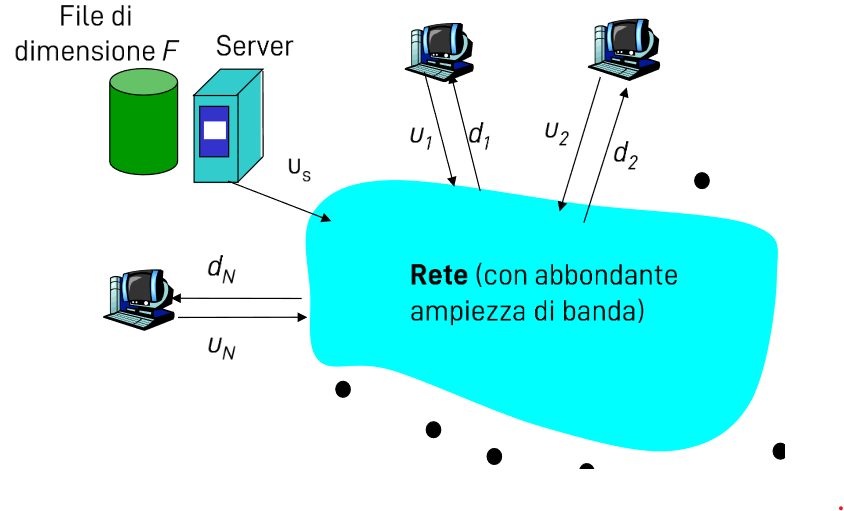
\includegraphics[width=0.5\textwidth]{02/reteP2P.png}
            \caption{Distribuzione di file in modalità \Acrshort*{P2P}}
        \end{figure}
        \paragraph{Domanda:} Tenendo a mente la soprastante figura, ci si può chiedere: Quanto tempo ci vuole per distribuire un file da un server a $ N $ \textit{peer}?\newline
        Consideriamo: \textbf{$U_s$} il \textit{bitrate} in uscita del collegamento di accesso del server, \textbf{$U_i$} bit rate di upload del collegamento di accesso dell \textit{i}-esimo \textit{peer} e \textit{$d_i$} il \textit{bitrate} di download del collegamento di accesso dell \textit{i}-esimo \textit{peer}.
        \paragraph{Soluzione \textit{server-client}} In una architettura \textit{server-client} il tempo di distribuzione è dato dal server che deve inviare $N$ copie moltiplicato per la dimensione del file $F$ il tutto diviso per il \textit{bitrate} in uscita del server $U_s$, quindi in formula: $T=\frac{N\cdot F}{U_s}$. Ora il client $i$-esimo impiega il tempo $F/d_i$ per scaricare il file. Per calcolare il tempo per distribuire il file $F$ su $N$ client è uguale al massimo tra il tempo impiegato dal server per la trasmissione ($U_s$) e dal tempo massimo impiegato da un client per scaricare il file ($d_i$), quindi $d_{cs} = \max\left\{\frac{F}{U_s}, \frac{F}{\min(d_i)}\right\}$. Notare come il tempo di distribuzione aumenta linearmente rispetto al numero di \textit{peer}.
        \paragraph{Soluzione per \Acrshort*{P2P}} In una architettura \Acrshort*{P2P} per calcolare il tempo di distribuzione dobbiamo prima sapere quanto tempo impiega \textit{server} per inviare la prima copia del file $ T_s = \frac{F}{U_s} $ e poi necessitiamo di sapere quanto tempo impiega l'\textit{i}-esimo client per scaricare il file: $T_i= \frac{F}{d_i} $. Dato che poi il \textit{peer} che ha scaricato il file poi può trasmetterlo a sua volta allora il puù veloce tasso di \textit{upload} è: $U_s+\sum_iU_i $. Il tempo totale è dato dunque dal massimo tra: tempo di invio prima copia, tempo massimo di un peer e il tempo di invio di tutte le copie ($\frac{NF}{U_s\sum_iU_i} $), quindi in modo formulare: $ d_{P2P}=\max\left\{\frac{F}{U_s}, \frac{F}{\min(d_i)}, \frac{NF}{U_S+\sum_iu_i}\right\} $. Notare come il tempo di distribuzione a meno di un tempo costate per l'invio della prima copia si riduce all'aumentare del numero di \textit{peer}.
        \subsubsection{BitTorrnet}
            \paragraph{Introduzione} Nel protocollo di \textit{BitTorrent} si usa la distribuzione di file in modo \Acrshort*{P2P} ma sono presenti dei \textit{server} detti \textit{tracker} che mantengono una lista di \textit{peer} partecipanti alla rete. Un nuovo \textit{peer} che vuole scaricare un file si connette al \textit{tracker} e ottiene la lista che stanno scaricando il file. Il \textit{peer} scarica il file da più \textit{peer} contemporaneamente, andando quindi a costituire una rete \textit{torrent}.
            \paragraph{Caratteristiche} I file vengono divisi in \textit{chunk} da $ 256kB $, quando un peer entra a far parte del torrent non possiede nessun \textit{chunk}, dunque si registra al server \textit{tracker} che gli assegna una lista di \textit{neighbors} ovvero vicini dai quali scaricherà i \textit{chunk} del file, quando un \textit{chunk} è scaricato il \textit{peer} lo condivide con gli altri alimentando l'effetto \textit{tit-for-tat}. Una volta che il file è scaricato nella sua completezza il \textit{peer} può lasciare la rete egoisticamente (\textit{leech}) o contribuire a questa (\textit{seeder})
    \subsection{Ricerca delle informazioni}
        I sistemi di tipo \Acrshort*{P2P} devono in qualche modo fornire un indice della posizione dei \textit{peer} e di in quali di questi si può trovare un particolare file, solitamente questo viene fatto attraverso una \textit{Distributed hash table}.
            \subsubsection{File sharing \textit{e-mule}}
                In un sistema come \textit{e-mule} l'indice tiene traccia dinamicamente della posizione dei file che i \textit{peer} condividono, questi condividono i file disponibili. Un nuovo \textit{peer} cerca nell'indice quello che vuole trovare e poi stabilisce una connessione diretta al \textit{peer} contenete il file cercato.
            \subsubsection{Messaggistica istantanea}
                Nel caso della messaggistica istantanea l'indice crea una corrispondenza tra utenti e posizione (\Acrshort*{IP}), quando un utente si registra all'applicazione informa il server della sua posizione, per inviare un messaggio ad un utente il \textit{peer} chiede al server la posizione dell'utente e poi stabilisce una connessione diretta.
            \subsubsection{Directory centralizzata}
                Nel caso di \textit{napster} invece quando un \textit{peer} si connette alla rete informa il server centrale del suo indirizzo \Acrshort*{IP} e del contenuto condiviso, se un altro \textit{peer} cerca il contenuto dal server centrale allora questo restituisce l'indirizzo \Acrshort*{IP} del \textit{peer} che condivide il file e il \textit{peer} può scaricare il file direttamente.
                \paragraph{Problemi} In primo luogo questa \textit{directory centralizzata} costituisce un \textit{Single point of failure}, inoltre essendo un solo punto questo è un importante \textit{bottleneck} infine se vengono condivisi file protetti da \textit{copyright} il server centrale ne è responsabile.
            \subsubsection{\textit{Query flooding}}
                Un sistema che adotta il \textit{query flooding} è completamente distribuito senza un server centrale, ogni \textit{peer} mantiene un indice locale dei file condivisi e quando un \textit{peer} cerca un file invia una \textit{query} a tutti i \textit{peer} vicini che se non hanno il file cercato inoltrano la \textit{query} ai loro vicini e così via. Questo sistema è molto efficiente ma può generare un grande traffico di rete. Una volta trovato il file viene istituita una connessione diretta \Acrshort*{TCP} tra i due \textit{peer}. Questo sistema è molto efficiente ma può generare un grande traffico di rete ed è soggetto ad attacchi di tipo \Acrshort*{DoS}, se viene richiesto un file inesistente la \textit{query} viene inoltrata a tutti i \textit{peer} della rete.
\section{Cloud Computing}
    \paragraph{Introduzione} Il \textit{cloud computing} prevede che uno o più \textit{server} reali, organizzati in una architettura ad alta affidabilità e fisicamente collocati in un \textit{data center} del fornitore del servizio. Il fornitore espone delle interfacce per elencare e gestire i propri servizi, un utente amministratore usa queste selezionando i servizi richiesti per accedervi o amministrarlo, infine un utente finale può accedere ai servizi tramite un'interfaccia web o un'applicazione.
    \paragraph{Criticità}
        \begin{itemize}
            \item \textbf{Privacy \& Sicurezza} - I dati sono memorizzati in un server remoto
            \item \textbf{Continuità del servizio} - I servizi sono soggetti a interruzioni e necessitano di connessione internet
            \item \textbf{Problemi internazionali di natura economico-politica} - I dati possono essere soggetti a leggi di paesi diversi
            \item \textbf{Difficoltà di migrazione} - I dati possono essere difficili da migrare una volta che sono stati caricati
        \end{itemize}
    \subsection[Content Delivery Network (\texttt{CND})]{\acrfull*{CDN}}
        \paragraph{Introduzione} Una \Acrshort*{CDN} è un sistema di server distribuiti che lavorano insieme per fornire contenuti web ad utenti finali con prestazioni elevate e alta affidabilità. Una \Acrshort*{CDN} è composta da \textit{server} detti \textit{edge server} che sono distribuiti in tutto il mondo, un \textit{server} centrale detto \textit{origin server} che contiene i contenuti originali e un \textit{server} detto \Acrshort*{DNS} \textit{server}
        \paragraph{Esempio} 
            \begin{itemize}
                \item Un utente richiede un oggetto
                \item Il \textit{\Acrshort*{DNS} server} determina il \textit{edge server \Acrshort*{CDN}} più vicino all'utente
                \item Il \textit{edge server} richiede l'oggetto all'\textit{origin server} e lo memorizza
                \item Il \textit{edge server} invia l'oggetto all'utente
                \item Il \textit{edge server} memorizza l'oggetto per un certo periodo di tempo
                \item Se un altro utente richiede lo stesso oggetto il \textit{edge server} lo invia direttamente
                \item Se l'oggetto non è più richiesto il \textit{edge server} lo elimina
                \item Se l'oggetto cambia il \textit{edge server} lo richiede all'\textit{origin server}
            \end{itemize}
    
    \paragraph{Conclusione} "There is no cloud, it's just someone else's computer"